\documentclass[a4paper]{jpconf}
\usepackage{graphicx}
\usepackage{lineno}
\usepackage{hyperref}
\usepackage{float}
\usepackage{lineno}
\linenumbers

\begin{document}
%\linenumbers



\title{Techniques and tools for measuring energy efficiency of scientific software applications}

\author{David Abdurachmanov$^1$, Peter Elmer$^2$, Giulio Eulisse$^3$, Robert Knight$^4$, Tapio Petteri Niemi$^5$, Jukka Nurminen$^6$, Filip Nyback$^6$, Goncalo Marques Pestana$^6$, Zhonghong Ou$^6$}

\address{$^1$ Digital Science and Computing Center, Faculty of Mathematics and Informatics, Vilnius University, Vilnius, Lithuania}
\address{$^2$ Department of Physics, Princeton University, Princeton, NJ 08540, USA}
\address{$^3$ Fermilab, Batavia, IL 60510, USA}
\address{$^4$ Research Computing, Office of Information Technology, Princeton University, Princeton, New Jersey 08540, USA}
\address{$^5$ Helsinki Institute of Physics, PO Box 64, FI-00014, Helsinki, Finland }
\address{$^6$ Aalto University, PO Box 11100, 00076 Aalto, Finland}

\ead{Peter.Elmer@cern.ch}

\begin{abstract}
As both High Performance Computing (HPC) and High Throughput Computing
(HTC) are sensitive to the rise of energy costs, energy-efficiency
has become a primary concern in scientific fields such as High
Energy Physics (HEP). There has been a growing interest in utilizing
low power architectures, such as ARM processors, to replace traditional
Intel x86 architectures. Nevertheless, even though such solutions
have been successfully used in mobile applications with low I/O and
memory demands, it is still unclear if they are suitable and more
energy-efficient in the scientific computing environment. Furthermore,
there is still lack of tools to derive and compare power consumption
for these types of workloads, and eventually to support software
optimizations for energy efficiency.

To that end, we have performed several physical and software-based
measurements of workloads from CERN running on ARM and Intel
architectures, to compare their power consumption and performance.
We leverage several profiling tools to extract different aspects
of the experiments, including hardware usage and software
characteristics. We report the results of these measurements and
the experience gained in developing a set of measurement techniques
and profiling tools to accurately assess the power consumption for
scientific workloads. [Version of~\today]
\end{abstract}

\section{Introduction}

 The most recent scientific applications have to process and store considerable 
volume of data. It is foreseeable that the volume of data will increase 
considerably in the future, as technology and requirements enhance. In addition
to the physical limitations in terms of power density, this phenomenon also
increase considerably the costs with energy in a HTC system. Thus, energy 
consumption has become a major concern amongst the scientific community. \\
 The Large Hadron Collider (LHC) ~\cite{LHCPAPER} at the European Laboratory for 
Particle Physics (CERN) in Geneva, Switzerland, is one of the scientific
projects which computational requirements are too massive for resources to be
 processed and held in one single infrastructure. Hence, data processing and 
storage 
are distributed across the Worldwide LHC Computing Grid (WLCG) ~\cite{WLHC}, 
which uses resources from 160 computer centers in 35 countries. The access to 
such computational resources have made possible CMS ~\cite{CMSDET} and ATLAS
 ~\cite{ATLAS} experiments to achieve important results, such as the discover of 
the Higgs Boson ~\cite{CMSHIGGS, ATLASHIGGS}. While enabling this and other
discoveries, the WLHC consumes massive amount of computational resources and, 
proportionally, energy. Only CMS experiment used approximately 80,000 to 100,000 
x86-64 cores of capacity in 2012, according to ~\cite{ACAT13ARM, CHEP13ARMPHI}.
In the future, with the improvement of the detector's luminosity, the dataset size
will increase by 2-3 orders of magnitude ~\cite{ACAT13ARM, CHEP13ARMPHI},
presenting even more challenges from the energy consumption point of view. \\

 In order to find and develop better solutions to improve energy efficiency in
High Energy Physics (HEP), it is
 important to understand how energy is used by the HEP systems themselves. There 
are 
few tools and techniques that facilitate researchers to reach that goal. Some of
these tools and techniques are outlined and described in this article.  \\
 As energy efficiency becomes a concern, new
solutions have been considered to develop energy efficient systems. One potential
solution is to replace the traditional Intel x86 architectures by low power
architectures such as ARM. A comparison of the energy efficiency between ARMv7 and 
x86 Intel architecture is conducted in this article. The experiments use CMS 
workloads and rely on the techniques and tools described earlier to perform the
measurements.\\

This article is structured as following. Firstly, we describe where is energy 
consumed in a HTC system. Secondly, we outline some of the tools and techniques 
available to measure and monitor energy consumption on HTC systems. Finally, we 
present the results of a comparison between ARMv7 and Intel Xeon architecture 
using CMS workloads.


\section{Tools and techniques for energy measurement}
As pictured in Figure 1, a HTC system is composed by several components.
It is important to grasp where and how energy is consumed by 
the system, so that researchers can trace, identify and improve energy 
bottlenecks. Therefore, given the specificities of those components, different 
types
of tools and techniques should be used to measure energy consumption, according
to what is suppose to measure.. 
In this section, we will outline and describe different approaches to measure 
energy consumption of the different components on a HTC system.  

\begin{figure}[ht!]
\centering
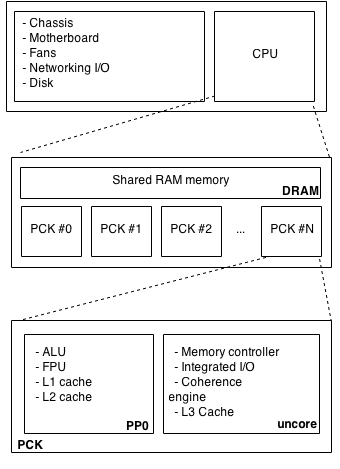
\includegraphics[width=70mm]{img/energy_model.png}
\caption{Components that contribute for power consumption in HPC}
\label{overflow}
\end{figure}

\subsection{External probing devices}

External probing devices measure the energy consumed by the whole system, 
without breaking it down in components pictured on Figure 1. 

\subsubsection{Noninvasive clamp meters and plug-in energy monitors} are probes 
that allow to measure electrical current pulled by the system without making 
physical contact or interfering with it. Generally, the accuracy of these tools
 is around 3\%, whereas its precision is in the order of seconds (Hz).

\subsubsection{Power distribution units} (PDU) are devices designed to distribute
electric power to systems. They are broadly used in server's rack and usually
have power monitoring capabilities embedded, which makes it useful for data
warehouses and big computing facilities. The accuracy and precision of such 
devices are similar to clamp meters described above.

\textit {can we generalize the accuracy and precision based on the tools
we used ? are there any references stating this ?}

\subsection{Internal probing chips}

\subsubsection{Chip monitors} perform energy monitoring from different modules
of the system on the chip (SoC). It allows energy measurements of fine grained
detail, being possible to individually monitor energy consumption of components 
such as core, dram, and others. Chip monitors are usually not included in the 
SoC from the manufacturer, but it can be added by third-party vendors. It can 
also be embedded by users, although it not a trivial task. In addition, usually
 the user has to develop its own code to read the results dumped by the chip. 
Commonly, the accuracy
of the measurements is high and the resolution is in the order of microseconds. 
An example of this chip monitors it the Texas Instrument INA231 (TI INA231)
\cite{TIINA231} current-churn and power monitor. 

\subsubsection{Running Average Power Limit}
(RAPL) provides a platform for monitoring and 
limiting power of  SoC. It is an Intel technology which was 
introduced initially on the Sandy Bridge processors. RAPL platform exposes 
chip's energy measurements via the MSR registers. According to ~\cite{RAPL1}, 
this technology offers power measurements of the system at a granularity 
impossible to reach before with other tools.

As documented by Intel in ~\cite{INTELMAN}, there are 3 different domains to 
sample energy consumed by different SoC components on a server. The domains are
 \textbf{package} (pck), which measures energy consumed by the system's sockets, 
\textbf{power plane 0} (pp0), which measures energy consumed by the CPU core, and \textbf{dram}, which 
accounts for the sum of energy consumed by memory in a given socket, excluding 
the core caches. The measurements are dumped in the MSR registers at a 
frequency of ~1 kHz and are exposed to the user via /dev/cpu/\textit{cpu\_nr}/msr. It 
is also possible to read and write data from the MSR register using Intel’s 
open source tool msr-tools ~\cite{MSRTOOLS}. 

In addition to power monitoring of the sockets, it can limit the power consumed 
by the different domains. This feature, usually referred as power capping, 
allows the user to define the average power consumption limit of a domain in a 
defined time window. For more information about RAPL’s features and 
configurations, refer to section 14.9.1 of Intel’s Developer’s manual 
~\cite{INTELMAN}.

The advantages of using RAPL for measuring power consumption are a straightforward and already installed tool to perform fine grained measurements of energy consumption on SoC and its components.

On the other hand, the drawbacks are lack of documentation available about the monitoring chip. To the knowledge of the authors, specifications such as error degrees, accuracy and implementation diagrams are not publicly available. In addition, the RAPL technology is vendor locked. Considering those two points, it is difficult to accurately compare and reason power measurements between SoCs from Intel and other vendors.



\subsection{Software based measuring tools}

There are software tools that provide insights about energy consumed by the
system. In addition, they can interact directly with the software. This
capability enables to map applications' code and energy consumption and help
developers to develop energy efficient applications. There are several examples
of software based measuring tools, such as powertop ~\cite{POWERTOP} and IgProf
\cite{igprof-web}, a general-purpose and open-source application profiler that 
was recently upgraded with energy measuring capabilities.

\subsection{IgProf}
IgProf is an application profiler that profiles mainly performance and memory usage. The profiler collects data about the resources an application uses. The resource of interest can be for example execution time, memory or file descriptors. The main idea behind profiling is to find the parts of the application where a resource is used the most, i.e.\@ possible bottlenecks. When the bottlenecks have been located, it makes sense to make optimisations where the bottlenecks are, because resource usage is usually not uniformly distributed over the whole application. \cite{igprof-web} \cite{tuura08} \cite{fowler02}

The profiler was available on the Intel x86 and x86-64 architectures, as well as on 32-bit ARM, but support for 64-bit ARM was missing. The port of IgProf to 64-bit ARM enables developers to evaluate how applications execute on the new architecture with regard to performance and memory usage.

A simple energy profiling module extends the functionality of IgProf. The energy profiling module is based on sampling and uses the PAPI library to obtain energy measurements from the RAPL (Running Average Power Limit) interface present on recent Intel processors. \cite{weaver12}

\begin{figure}[htb]
  \begin{center}
    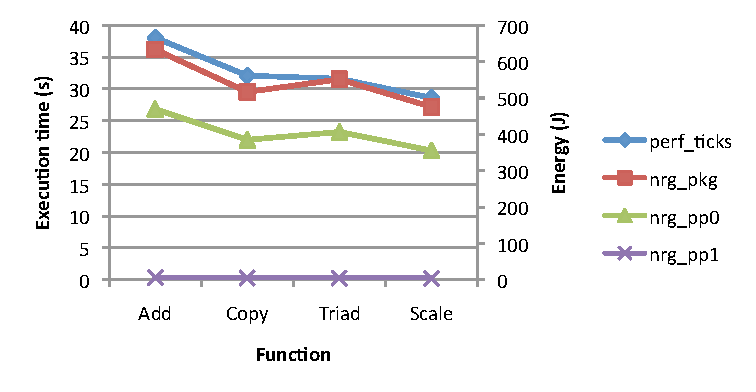
\includegraphics{img/stream-pp-np.pdf}
  \end{center}
  \vspace{-20pt}
  \caption{The results of performance and energy profiling of the stream tool.}
  \label{fig:stream-pp-np} 
\end{figure}

Figure \ref{fig:stream-pp-np} shows the results from performance and energy profiling of the \emph{stream} benchmarking tool. The X-axis describes the four main functions contributing to the execution time and energy consumption of the stream tool: Add, Copy, Triad and Scale. The left scale of the Y-axis and the perf\_ticks series describe the execution time spent in each function, whereas the right scale of the Y-axis and the nrg\_pkg, nrg\_pp0 and nrg\_pp1 series describe the amount of energy spent in each function. The energy consumption of the processor package domain and the power plane 0 (describing the CPU cores) seem to follow the time spent in the functions, whereas the energy consumption of power plane 1 (describing the GPU) seems to be fairly constant. \cite{stream-web}

The profiling results of a simple single-threaded application seem to show a correlation between the execution time and the energy spent in a function. The energy profiling module is, however, still rather limited; e.g.\@ it does not seem to profile multi-threaded applications correctly. 

\section{Use case}
In this section, we demonstrate the potentialities of some of the tools 
presented in Section 2. To that end, we perform several measurements of workloads
from CERN, running in different architectures. The workloads used in the 
experiment run on top of Intel architectures, traditionally used in HTC and data
 centers, and ARM architectures. ARM architecture, initially developed for mobile
 devices, has been considered \cite{ACAT13ARM, CHEP13ARMPHI} as a potential 
alternative to Intel in HTC, given its energy efficient computing. We also 
present brief comparison between ARM and Intel architectures from the energy
consumption perspective, based on the results obtained. \\

\subsection{Tools and techniques}
On Intel architecture, we used RAPL technology to
perform measurements of the energy consumed by the package, dram and cores (see
Figure 1). The external measurements were performed using a rack PDU, which 
provides an online API to gather the energy consumed by the system on the rack 
at a sampling rate of around 1s.

As for the ARM machine, we used the Texas Instrument power monitor chip 
TI INA231 (see section 2.2.1) which allows reading of the energy consumed by the
cores and dram at a sampling rate of microseconds. The chip was embedded in the 
board (see Figure 3) from the vendor. For the external measurements, we used
an external plug-in power monitor with a computer interface for gathering and
storing the results.

\subsection{Experiment setup}
The workload used for the experiments was ParfullCMS [?]. It consists
of a multi-threaded Geant4 [?] benchmark application and uses the complex
CMS geometry to simulate the offline tasks of CMS software. Using ParfulCMS, 
we ran CMS reconstruction tasks
on both Intel and ARM machines (see Figure 3). The workflow was run several
times for different number of threads in each machine. The number of threads
running in each experiment is according to the number of the cores of the
machines. The machine's specifications can be seen in the Figure 3. 

\subsection{Analysis}

\begin{figure}[H]
\centering
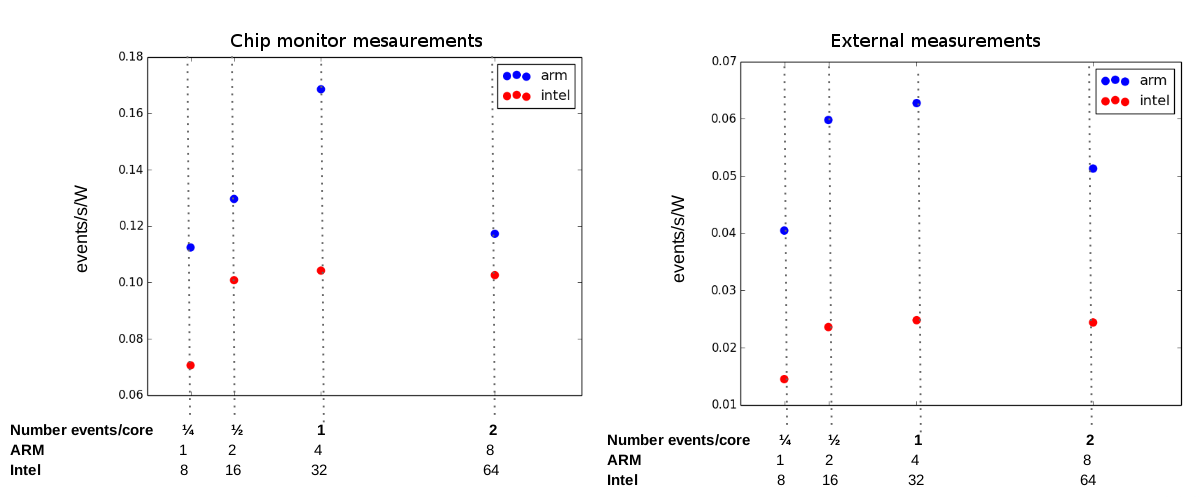
\includegraphics[width=170mm]{img/results1.png}
\caption{Chip monitor and external measurements results}
\label{overflow}
\end{figure}

As expected, the ARM architecture shows better results from the energy efficiency
 perspective than Intel in all the experiments performed. Also as expected, both 
architectures do not performs better when overcommitted (more threads than the
physical number of cores). An interesting feature of the ARM results when 
overcommitted (8 threads) is the deterioration of the energy performance. It
would be expected a behaviour similar to Intel in same circumstances. However, due
to the relatively modest amount of available DRAM (see Figure 3), the machine
started swapping. The memory swapping takes time and resources and, thus, 
consumes more energy.

\section{Conclusions}
Energy efficiency has become a major concern on HTC, given the large amount of
resources - and thus energy - that recent experiments require. The LHC is
a relevant example of the need for energy efficiency facilities, given its present
requirements and costs constrains. The urgency for energy efficiency brings up the
need for accurately measure the different components of a HTC system. The goal is,
thus, to understand how and where energy is consumed and improve the overall 
energy efficiency. However, HTC systems are complex and composed of different 
components. Therefore, we presented examples of techniques and tools that provide
better knowledge of how and where energy is consumed from different perspectives
and granularities. In addition, IgProf, an open source profiling tool, was 
further developed to run on 64-bit ARM and include energy profiler capabilities. On 
the endeavor to achieve better energy performance on HTC, ARM architecture has
been considered to replace the traditional Intel machines. Therefore, and in 
order to apply some energy measurement techniques studied in this article, we
performed a simple comparison between ARMv7 and Intel architectures. The results 
confirm the potential of ARMv7 for efficient HTC systems.   


\section*{Acknowledgements}
This work was partially supported by the National Science Foundation, under
Cooperative Agreement PHY-1120138, and by the U.S. Department of Energy.

\section*{References}

\bibliographystyle{unsrt}
\bibliography{acat2014-energy-efficiency}

\end{document}
